\chapter{Analiza}
\label{ch:analiza}

Every number reported in this chapter is produced by a measured run.

\section{Metodologija}
\label{sec:metodologija}

\paragraph{Hardver: cross-vendor postavka.} The central evaluation compares the identical pipeline on
two current-generation GPUs from different vendors: an AMD Radeon RX 9070 XT (RDNA4) and an NVIDIA
GeForce RTX 5070 (Blackwell), specified in Table~\ref{tab:gpus}. Both run the same engine binary, the
same SPIR-V shaders, the same render graph, and the same scene and settings; the only variable is the
selected physical device, which is the fairness basis: any difference in timing is due to the
hardware and its driver rather than to a different code path, and a quality divergence would point at
a non-determinism worth investigating rather than at a real difference. The one documented exception
to the identical-code-path claim is opacity micromap support.

\begin{table}[tbp]
\caption{GPU-ovi u cross-vendor pore\dj enju, prema zvani\v{c}nim specifikacijama proizvo\dj a\v{c}a
(AMD, NVIDIA) i verzijama drajvera sa test ma\v{s}ine.}
\label{tab:gpus}
\centering
\begin{tabularx}{\textwidth}{l >{\raggedright\arraybackslash}X >{\raggedright\arraybackslash}X}
\toprule
 & AMD RX 9070 XT & NVIDIA RTX 5070 \\
\midrule
Arhitektura            & RDNA4 (Navi 48) & Blackwell (GB205) \\
Compute jedinice / SM  & 64 CU, 4096 stream procesora & 48 SM, 6144 CUDA jezgara \\
RT akceleratori        & 64 (3. generacija) & 48 \\
Takt (boost)           & 2970 MHz & 2512 MHz \\
Memorija / propusnost  & 16 GB GDDR6, 640 GB/s & 12 GB GDDR7, 672 GB/s \\
TDP (TBP / TGP)        & 304 W & 250 W \\
Drajver / OS           & 32.0.31035.1003, Windows 11 Pro (build 26100) & 32.0.15.9186, Windows 11 Pro (build 26100) \\
\bottomrule
\end{tabularx}
\end{table}

\paragraph{Nesaglasje u podr\v{s}ci za OMM.} Sponza carries three MASK-mode (alpha-cutout) materials, which
trace through the opacity-micromap BLAS on a device exposing \texttt{VK\_EXT\_opacity\_micromap} and
through the any-hit alpha-test fallback otherwise (Section~\ref{sec:accel}). The RTX 5070 driver
exposes the extension and the 9070 XT driver does not, despite comparable hardware capability, so the
two vendors resolve masked geometry through genuinely different acceleration-structure code here. The
disparity only changes how a masked microtriangle is classified during traversal, not ray direction,
hit position or shading, so it cannot explain a quality-metric difference. It is a small,
one-directional, driver-dependent contributor to the per-effect GPU-ms gap wherever a ray hits cutout
geometry, and this evaluation does not isolate it further.

\paragraph{Scena i kontrole.} The test scene is Sponza, a standard interior with strong indirect
bounce, lit by five enabled lights: four point torches and one directional sun. Three spot lights and
two further point lights are authored but disabled, and the distinction matters because the default
shadow path costs one ray per light per pixel.

One property of the raster path bounds every technique that uses it: the engine allocates at most two
omni shadow maps (\texttt{MAX\_SHADOW\_POINTS}, six depth passes each), so two of the four enabled
point lights render unshadowed. Ray-traced shadows have no such cap, tracing one ray per light, so
every technique in Table~\ref{tab:quality} except \texttt{sve RT} sits on a weaker shadow baseline
than a renderer without that limit, which flatters the ray-traced side. The effect is bounded and
small: the shadow technique alone moves PSNR 0.65 dB of the 15.68 dB between raster and all effects,
and FLIP 0.024 of 0.349, so the lift in Section~\ref{sec:poredjenje} is dominated by global
illumination rather than by this cap.

Every measurement in this chapter renders at
$1915 \times 1064$, with the camera held static for every A/B comparison, since a moving camera
desynchronizes the frame sequence between two runs and fabricates differences that are timing
artifacts. The shader cache is cleared before any GPU metric is trusted, since a stale cache produces
nondeterministic results, and persisted console variables are ignored during a benchmark run, so a
leftover setting cannot silently change the configuration. Performance baselines are per-machine and
per-resolution, because absolute milliseconds are not comparable across GPUs or output sizes.

\paragraph{Merenje performansi.} GPU time comes from the per-pass timestamp scopes and the
\texttt{perf-bench} harness of Section~\ref{sec:alati}, averaged over a fixed frame budget once a
steady state has been detected rather than assumed: frame time takes about fifty frames to settle on
this scene, so a fixed short warmup would average part of the clock ramp into the result, by an
amount depending on how warm the machine already was and with nothing in the output to indicate it.
The benchmark sweeps a fixed
matrix of configurations, \texttt{rt-off} $\rightarrow$ \texttt{shadows} $\rightarrow$ \texttt{+ao}
$\rightarrow$ \texttt{+refl} $\rightarrow$ \texttt{+gi}, enabling one more effect at each step, so the
cost of an effect is the difference between adjacent configurations. A difference rather than an
isolated timing, because effects share fixed work (acceleration structure built once, G-buffer filled
once, tonemap run once): timing an effect alone would charge it for all of that, and the four figures
would then sum to considerably more than the frame costs.
The difference is taken on \emph{total} GPU time rather than on one pass scope, since
inline shadows are traced inside the Forward pass and have none of their own; the other three
effects do, and are reported as whole-frame deltas anyway for consistency. A
trailing \texttt{ssgi} configuration swaps ray-traced GI for the screen-space producer on top
of \texttt{+refl} and is diffed against \texttt{+refl}, since the two are alternatives rather than
cumulative. Timestamps are converted with each device's timestamp period, so
per-pass times are comparable across vendors, and both GPUs are reported side by side rather
than against a single-machine baseline, since the cross-vendor comparison is itself the
measurement.

\paragraph{Merenje kvaliteta.} Reconstruction quality is measured by \texttt{quality-bench} against
the converged path-traced reference of Section~\ref{sec:pathtracer}. Each real-time technique's
tonemapped present is scored against it by \textbf{FLIP} (perceptual), \textbf{PSNR} and
\textbf{SSIM}. FLIP is primary because it models what a human observer notices rather than raw
per-pixel error; PSNR structurally favours a blurrier image and SSIM compares local structure rather
than absolute values, so all three are reported and no single metric's bias decides a conclusion.
Scores are averaged over three fixed orientations from one interior position (down the nave, tilted
to the floor, tilted to the upper gallery), chosen to stress ambient occlusion, global illumination
and reflections differently, so a single framing cannot bias the result. Each capture is bilinearly
resampled to a canonical $1024 \times 576$ first, so a window-size difference between runs cannot
silently change a score. Quality figures elsewhere in this chapter are
the RX 9070 XT's; Section~\ref{sec:cross-vendor-quality} captures the whole matrix on the RTX 5070 as
well.

\section{Cena po efektu (GPU ms)}
\label{sec:cena}

\begin{table}[tbp]
\caption{Cena po efektu (GPU ms) na cross-vendor paru RX 9070 XT / RTX 5070, pri rezoluciji
$\perfWidth \times \perfHeight$ i fiksiranoj pozi kamere, prosek preko \perfFrames{} frejmova.
\texttt{rt-off} je ukupno GPU vreme bez RT efekata; svaki naredni red je dodatak (delta) tog efekta u
odnosu na prethodnu konfiguraciju. Red \texttt{ssgi} je alternativa za \texttt{+gi} (screen-space GI
umesto RT GI) i pore\dj en je sa \texttt{+refl}, ne kumulativno sa \texttt{+gi}. Sve vrednosti se
generi\v{s}u iz committovanih baseline-a skriptom \texttt{tools/gen\_perf\_tables.py}.}
\label{tab:cena}
\centering
\begin{tabular}{llrr}
\toprule
Configuration & Effect & ms (9070 XT) & ms (5070) \\
\midrule
\texttt{rt-off}   & baseline (total) & 2.274 & 1.347 \\
\texttt{+shadows} & shadows & 2.272 & 1.294 \\
\texttt{+ao} & ambient occlusion & 0.817 & 0.728 \\
\texttt{+refl} & reflections & 1.756 & 1.291 \\
\texttt{+gi} & global illumination (RT) & 1.705 & 1.309 \\
\midrule
\texttt{+gi} & \textbf{total, all effects} & \textbf{8.824} & \textbf{5.970} \\
\midrule
\texttt{ssgi} & screen-space GI (alternative to +gi) & 0.739 & 0.667 \\
\bottomrule
\end{tabular}

\end{table}

In Table~\ref{tab:cena} the per-effect rows are differences, although the total is the measured
whole-frame time of the \texttt{+gi} configuration rather than their sum, so rounding cannot
accumulate. Table~\ref{tab:pass-cost} breaks that same frame down by pass.

\begin{table}[tbp]
\caption{Najskuplji prolazi u \texttt{+gi} konfiguraciji (GPU ms, prosek preko \perfFrames{}
frejmova). \texttt{Forward} sadr\v{z}i i inline RT senke, pa nema zaseban scope. GI i AO filtriraju u
polovi\v{c}noj rezoluciji. Prolazi za denoise-ovanje refleksija ne pojavljuju se u tabeli jer se vi\v{s}e
ne izvr\v{s}avaju: \texttt{render.reflections.denoise.iterations} je sada 0
(odeljak~\ref{sec:denoise-eval}).}
\label{tab:pass-cost}
\centering
\begin{tabular}{lrr}
\toprule
Pass & ms (9070 XT) & ms (5070) \\
\midrule
\texttt{Forward} (includes inline shadows) & 4.444 & 2.396 \\
\texttt{Reflection} & 1.495 & 1.136 \\
\texttt{GI} & 1.076 & 0.725 \\
\texttt{GIDenoise*} & 0.329 & 0.317 \\
\texttt{AODenoise*} & 0.330 & 0.309 \\
\texttt{AO} & 0.170 & 0.199 \\
\texttt{DepthNormal} & 0.142 & 0.231 \\
\texttt{TemporalResolve} (TAA) & 0.177 & 0.090 \\
\bottomrule
\end{tabular}

\end{table}


\begin{figure}[tbp]
\centering
\begin{tikzpicture}
\begin{axis}[width=0.88\textwidth, height=6.4cm,
  xlabel={konfiguracija}, ylabel={ukupno GPU (ms)},
  xtick={0,1,2,3,4},
  xticklabels={\texttt{rt-off},\texttt{shadows},\texttt{+ao},\texttt{+refl},\texttt{+gi}},
  ymin=0, grid=major, grid style={black!12},
  tick label style={font=\small}, label style={font=\small},
  legend style={at={(0.02,0.98)}, anchor=north west, font=\small, draw=black!30}]
\addplot[thick, mark=*] table[col sep=tab, x=i, y=amd] {data/ladder.dat};
\addplot[thick, mark=square*, dashed] table[col sep=tab, x=i, y=nv] {data/ladder.dat};
\legend{RX 9070 XT, RTX 5070}
\end{axis}
\end{tikzpicture}
\caption[Kumulativno GPU vreme kroz lestvicu konfiguracija]{Ukupno GPU vreme kroz lestvicu, gde svaka
sledeca konfiguracija uklju\v{c}uje jo\v{s} jedan efekat. Nagib segmenta je cena tog efekta. Obe
kartice rastu monotono, ali AMD kre\'ce vi\v{s}e i raste br\v{z}e, pa se razmak \v{s}iri sa 0.93 ms na
\texttt{rt-off} do 2.85 ms na \texttt{+gi}.}
\label{fig:ladder}
\end{figure}

\begin{figure}[tbp]
\centering
\begin{tikzpicture}
\begin{axis}[xbar, bar width=5pt, width=0.62\textwidth, height=9.5cm,
  xlabel={odnos AMD / NVIDIA (GPU ms)},
  xmin=0, xmax=2.2, y dir=reverse,
  ytick={0,...,15}, yticklabels from table={data/passcost-vendor.dat}{pass},
  yticklabel style={font=\footnotesize}, tick label style={font=\small},
  label style={font=\small}, grid=major, grid style={black!12},
  nodes near coords, nodes near coords style={font=\tiny, /pgf/number format/fixed,
    /pgf/number format/precision=2}]
\addplot[fill=black!18, draw=black!55] table[col sep=tab, x=ratio, y expr=\coordindex]
  {data/passcost-vendor.dat};
\draw[dashed, black!60] (axis cs:1,-1) -- (axis cs:1,16);
\end{axis}
\end{tikzpicture}
\caption[Odnos cene po prolazu izme\dj u proizvo\dj a\v{c}a]{Cena svakog prolaza na AMD-u podeljena
cenom istog prolaza na NVIDIA-i, u \texttt{+gi} konfiguraciji. Isprekidana linija je paritet. Desno od
nje NVIDIA je br\v{z}a, levo AMD. Raspon od 0.62 do 1.96 pokazuje da razlika nije jedan globalni
faktor takta: \texttt{Forward} (koji nosi inline senke) i \texttt{TemporalResolve} idu jako u korist
NVIDIA-e, dok tre\'ca a-trous iteracija i \texttt{DepthNormal} idu u korist AMD-a.}
\label{fig:vendor-ratio}
\end{figure}

The two cards do not agree on which effect is most expensive. On the RX 9070 XT shadows dominate at
\perfEffShadowsAMD{} ms, well clear of reflections and global illumination. On the RTX 5070 those
same three fall within \perfNVSpread{} ms of each other, inside the run-to-run spread, so on that
card they are indistinguishable in cost. Ambient occlusion is cheapest on both. Together the four add
\perfFourEffectsAMD{} ms (9070 XT) and \perfFourEffectsNV{} ms (5070) over their respective
baselines, for measured real-time totals of \perfTotalAMD{} ms (\perfBaseAMD{} ms baseline) and
\perfTotalNV{} ms (\perfBaseNV{} ms baseline).

The half-resolution trace plus denoise is what keeps GI and AO cheap despite their hemispheric
gather. On both cards the screen-space GI producer is cheaper than ray-traced GI at the same rung
(9070 XT 0.739 against 1.705 ms; RTX 5070 0.667 against 1.309 ms), the expected
screen-space-versus-ray-traced cost tradeoff, whose quality side is Section~\ref{sec:poredjenje}.

Reflections are no longer the most expensive effect, and the reason is a deliberate default change
rather than an optimisation: the reflection à-trous filter measured net-negative and now runs zero
iterations (Section~\ref{sec:denoise-eval}), removing a full-resolution three-pass chain worth roughly
1.1 ms. They remain the only effect tracing at full resolution, so their trace alone (1.495 ms on the
9070 XT) costs more than the half-resolution GI trace. Ambient occlusion is cheapest despite casting
more rays per pixel, because those rays are short (bounded by \texttt{render.ao.radius}) and
terminate on the first hit, while a reflection ray can traverse the whole scene and then shade what
it finds.

Shadows have no scope of their own, so their cost has to be read across configurations. Between
\texttt{rt-off} and \texttt{shadows} on the 9070 XT the Forward pass grows by 3.482 ms while the
raster shadow-map passes disappear entirely, returning 1.056 ms (\texttt{Shadow} 0.107 and
\texttt{PointShadows} 0.949). Those two terms give 2.426 ms against a measured whole-frame delta of
2.272 ms; the remaining 0.154 ms is every other pass shrinking slightly at once, the signature of a
clock shift rather than of real savings, consistent with \texttt{rt-off} being the noise-dominated
configuration on this adapter (8.3\% run-to-run spread against under 1\% for the others). The
whole-frame difference is the number to quote, since the per-pass terms do not close.

\begin{figure}[tbp]
\centering
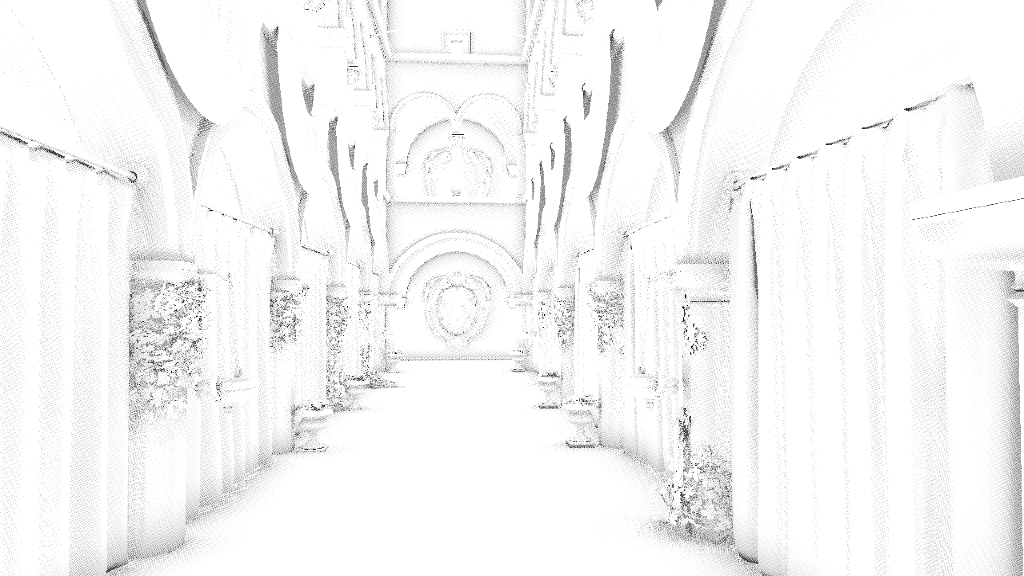
\includegraphics[width=0.48\textwidth]{figures/dbg_ao.png}\hfill%
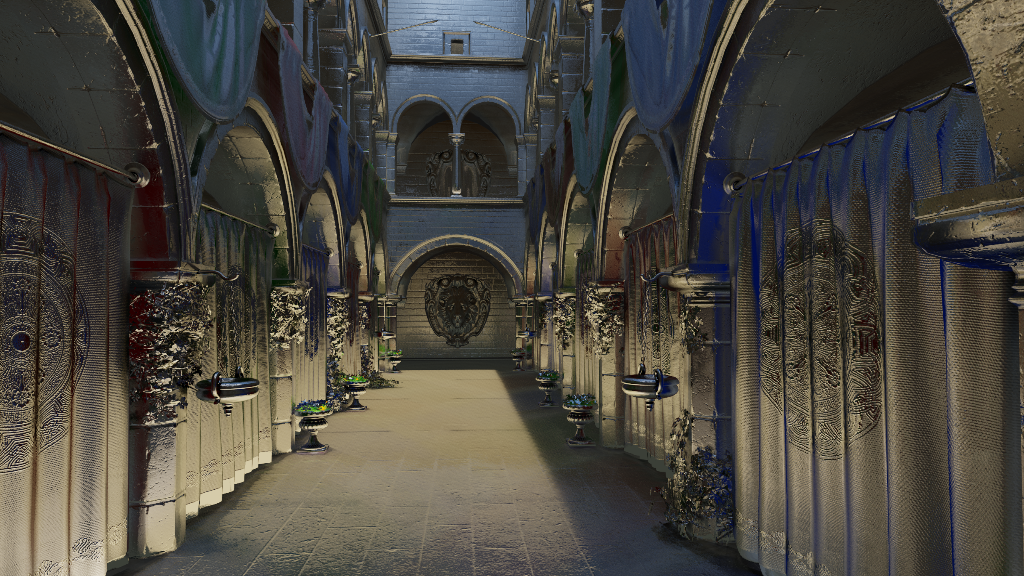
\includegraphics[width=0.48\textwidth]{figures/dbg_refl.png}

\vspace{5pt}

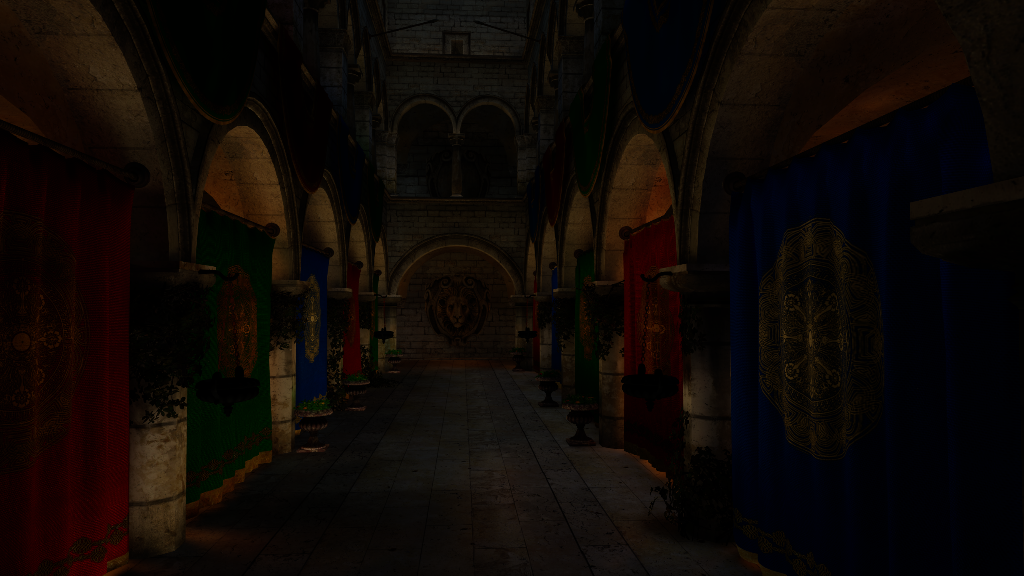
\includegraphics[width=0.48\textwidth]{figures/dbg_gi.png}\hfill%
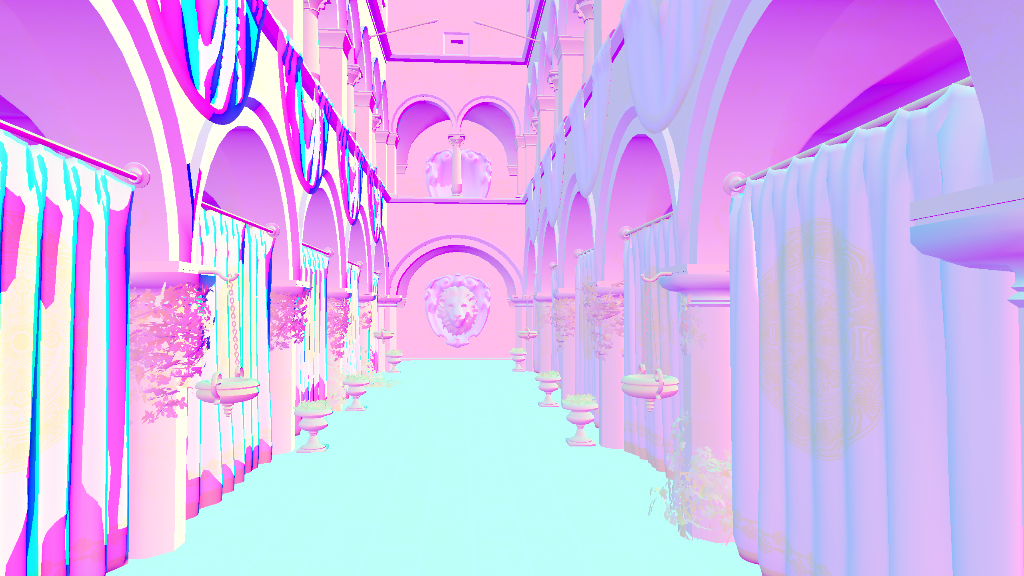
\includegraphics[width=0.48\textwidth]{figures/dbg_normals.png}
\caption{Pojedina\v{c}ni signali izolovani preko \texttt{render.debugview}, ista scena i kamera:
ambijentalna okluzija (gore levo), reflektovana radijansa (gore desno), indirektni GI \v{c}lan
(dole levo) i normale iz G-buffer-a (dole desno). Prikazani su sirovi me\dj urezultati pre
kombinovanja u forward prolazu, a ne gotova slika.}
\label{fig:effect-gallery}
\end{figure}

Toggling shadows, ambient occlusion or reflections individually moves the final image by a mean of
only 2.1 to 2.5 levels out of 255 at this viewpoint, while global illumination moves it by 23.9. The
ambient-occlusion buffer is close to white over most of the frame because Sponza's atrium is open, so
occlusion is confined to the arcade vaults and the column bases; the raw GI term is dim in absolute
terms yet carries the colour bleeding (the red and green drapes tinting the stone beside them) that a
constant ambient cannot reproduce.

\section{Dve strategije za senke: inline naspram stohasti\v{c}ke}
\label{sec:analiza-shadow-strategy}

The two shadow strategies of Section~\ref{sec:senke} have differently shaped cost curves: the default
inline path traces one ray per light per pixel inside the forward shader, while the stochastic path
picks one light per pixel by resampled importance sampling and reconstructs the result with the
shared denoiser.

\begin{table}[tbp]
\caption{Dve strategije za senke na istoj sceni sa pet upaljenih svetala (GPU ms, dodatak u odnosu na
\texttt{rt-off}).}
\label{tab:shadow-strategy}
\centering
\begin{tabular}{lrr}
\toprule
Strategy & ms (9070 XT) & ms (5070) \\
\midrule
inline, per light (default) & 2.272 & 1.294 \\
stochastic, RIS + denoiser & 1.723 & 3.362 \\
\bottomrule
\end{tabular}

\end{table}

The two cards disagree about which strategy is cheaper. On the RX 9070 XT the stochastic path wins,
1.723 ms against 2.272 ms. On the RTX 5070 it loses badly, 3.362 ms against 1.294 ms, a factor of
2.6.

The stochastic path replaces per-light rays with one importance-sampled ray plus a reconstruction
chain, trading ray count for filter cost, which pays exactly when rays are expensive relative to
filtering. On the 5070 they are not: dedicated traversal hardware makes the twenty coherent inline rays of a five-light scene
cheap enough that paying a temporal pass, three à-trous iterations, and an upsample to avoid them is a
net loss. On the 9070 XT, where traversal is driven by shader instructions and competes with shading
for the same execution resources (Section~\ref{sec:accel-pregled}), the same trade pays.

The choice of shadow technique is therefore a property of the target architecture: a renderer that
hard-codes either strategy is wrong on one of these two cards, and a single-vendor evaluation cannot
see that.

Two caveats bound the claim. The stochastic path's cost is nearly independent of light count while the
inline path's grows with it, so five lights is one point on two curves that must cross somewhere; this
scene cannot show where. And the stochastic producer is experimental and off by default, with known
artifacts under camera motion where two point lights overlap, so these are the numbers of a prototype
rather than of a shipping technique.

\section{Broj zrakova naspram kvaliteta i brzine}
\label{sec:raycount}

The GI ray count per pixel is swept through the full pipeline (denoiser and temporal resolve enabled,
settled over 90 frames, RX 9070 XT), scoring reconstruction quality against the path-traced reference
and GPU time against the ray count.

\begin{table}[htb]
\centering
\caption{GI kvalitet i GPU cena u funkciji broja zraka po pikselu (denoiser i temporalni resolve
uklju\v{c}eni, RX 9070 XT).}
\label{tab:raycount}
\begin{tabular}{@{}rrrrr@{}}
\toprule
Rays/pixel & PSNR (dB) & SSIM & FLIP & GPU total (ms) \\
\midrule
1 & 24.52 & 0.7356 & 0.1486 & 3.51 \\
2 & 24.65 & 0.7395 & 0.1449 & 3.85 \\
4 & 24.67 & 0.7407 & 0.1458 & 4.28 \\
8 & 24.73 & 0.7432 & 0.1433 & 6.43 \\
\bottomrule
\end{tabular}

\end{table}

The knee sits at 1 ray per pixel. Going from 1 to 8 rays costs \rcGpuPct\% more GPU time
(\rcGpuLow{} to \rcGpuHigh{} ms) for a \rcPsnrGain{} dB PSNR gain and a FLIP improvement from
\rcFlipLow{} to \rcFlipHigh{}, both within run-to-run noise on
this metric. The denoiser and temporal accumulation already recover most of the achievable quality
from a single ray, so additional samples per pixel are not where this engine's ray budget should go.
This is consistent with the SVGF design goal (spatiotemporal
filtering to make 1 sample per pixel viable) rather than a property specific to this
implementation. Figure~\ref{fig:spp-sweep} shows the raw noise this filtering masks, captured with the
GI spatial denoiser, the GI temporal accumulation and TAA disabled, at a fixed 30-frame cap.
Disabling TAA is what makes the figure honest: TAA is itself a temporal
accumulator, so with it enabled the capture settles into the same smoothness as the denoised image and
the ray count appears to make no difference at all.

Quantifying that needs a measure of per-pixel roughness. Define the \emph{high-frequency energy} of an
image as the mean absolute difference between vertically adjacent pixels of its grayscale channel,
$\frac{1}{(H-1)W}\sum_{y,x} |g_{y+1,x} - g_{y,x}|$, computed on the 8-bit tonemapped capture; noise
raises it, blur lowers it, and it can be recomputed from the committed figures. With TAA enabled, one
ray per pixel and the fully denoised image both score 5.9, which is the measurement saying the figure
would show nothing. With TAA disabled the ray count separates cleanly: 10.8, 9.1, 8.1, and 7.3 for
one, two, four, and eight rays per pixel, monotonically approaching the reference as the sample count
rises.

\begin{figure}[tbp]
\centering
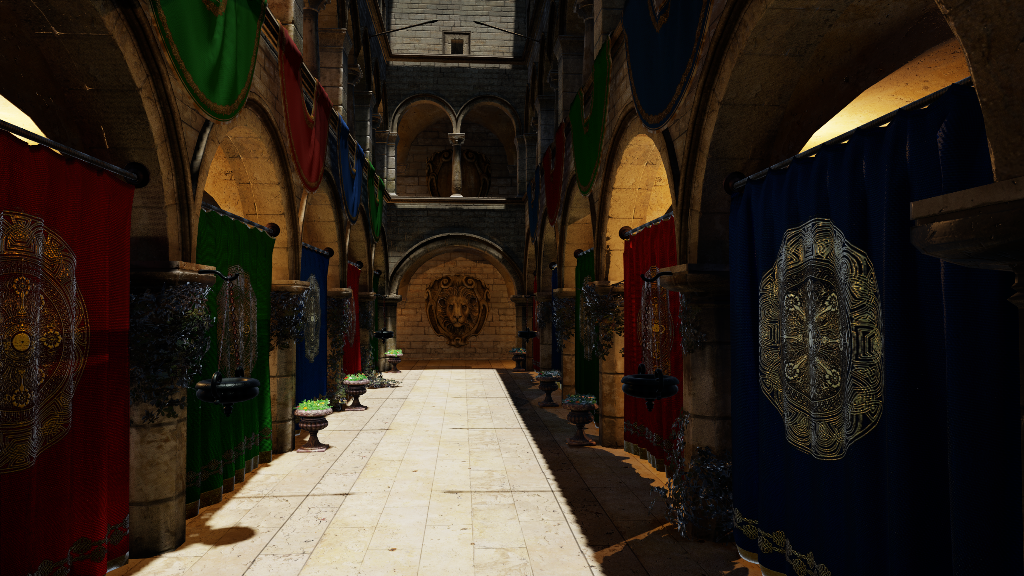
\includegraphics[width=0.48\textwidth]{figures/spp_sweep_1.png}\hfill%
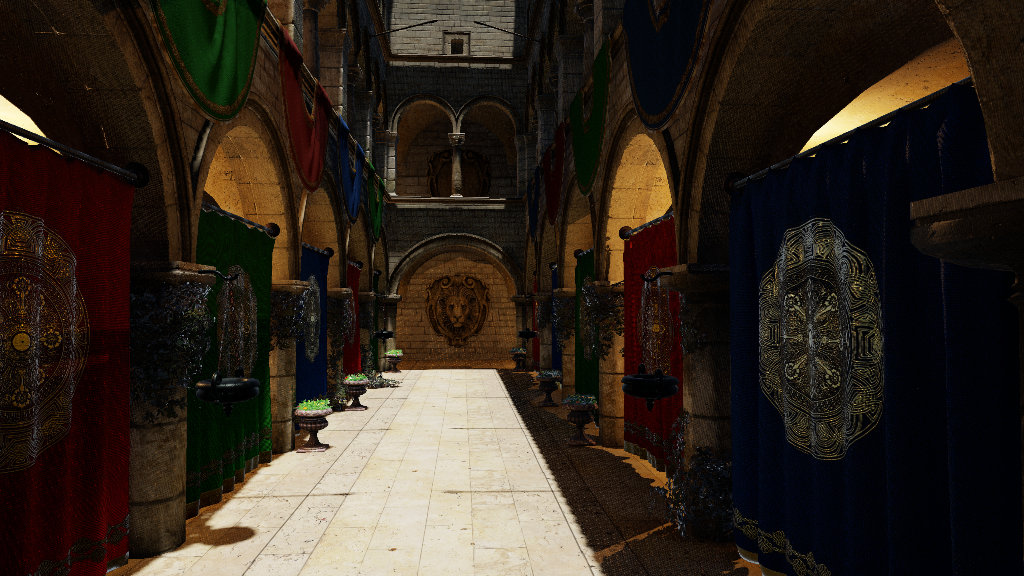
\includegraphics[width=0.48\textwidth]{figures/spp_sweep_8.png}
\caption{Uticaj broja zraka po pikselu na \v{s}um pre denoise-a, pre temporalnog resolve-a i bez TAA
(GI; levo 1 zrak, desno 8 zrakova po pikselu): vi\v{s}e zraka konvergira ka referenci, uz
proporcionalno ve\'cu cenu (Tabela~\ref{tab:raycount}).}
\label{fig:spp-sweep}
\end{figure}

\section{Polovi\v{c}na naspram pune rezolucije}
\label{sec:halfres}

Tracing the two hemispheric gather effects at half resolution is the single largest cost decision in
the renderer (Section~\ref{sec:rendergraph}). Setting \texttt{render.gi.scale} and \texttt{render.ao.scale} to 1.0 turns it off, changing nothing else, so
the two configurations differ in exactly one variable.

\begin{table}[tbp]
\caption{Polovi\v{c}na naspram pune rezolucije za GI i AO trasiranje (RX 9070 XT). Vreme je ukupno GPU
vreme \texttt{+gi} konfiguracije; kvalitet je meren iz atrijumskog pogleda naspram konvergirane
path-traced reference.}
\label{tab:halfres}
\centering
\begin{tabular}{lrrr}
\toprule
 & half (0.5) & full (1.0) & difference \\
\midrule
Total GPU (ms) & 8.67 & 13.34 & $+54\%$ \\
\texttt{GI} pass (ms) & 1.07 & 4.12 & $\times 3.8$ \\
\texttt{AO} pass (ms) & 0.17 & 0.63 & $\times 3.8$ \\
\midrule
PSNR (dB) & 29.58 & 29.58 & $+0.00$ \\
SSIM & 0.8702 & 0.8710 & $+0.0008$ \\
FLIP & 0.1027 & 0.1025 & $-0.0002$ \\
\bottomrule
\end{tabular}

\end{table}

Full-resolution tracing costs \hrDeltaMs{} ms more per frame, a \hrDeltaPct\% increase on a
\hrHalfTotal{} ms budget, and returns \hrPsnrGain{} dB of PSNR: the two configurations are identical
to the second decimal. SSIM and FLIP move by 0.0008 and 0.0002, both far inside the run-to-run
spread. The reading is not \rqt{full resolution is slightly better} but \rqt{the measurement cannot
distinguish them at all}.

The reason is that the denoiser is the binding constraint, not the sample grid. Both configurations
feed the same à-trous filter, whose edge-stopping kernel already blurs over a neighbourhood wider than
the factor of two separating them; the extra samples are averaged away by the very filter that makes
the half-resolution result usable. The half-resolution plus bilateral-upsample pattern is therefore
close to free rather than a quality compromise accepted for speed.

Figure~\ref{fig:halfres-buffer} shows the raw GI irradiance under both settings, taken through the
debug view that bypasses the upsample, denoiser and composite. The half-resolution buffer carries
44\% more high-frequency energy by the roughness proxy of Section~\ref{sec:raycount} (41.68
against 28.91). That proxy is reproducible where the per-pixel difference is not: a second
full-resolution capture with identical settings scores 28.85, within 0.2\%, while differing from the
first by 18.3 grey levels per pixel simply because the two traces drew different random samples. So
the per-pixel gap of 35.4 between the half- and full-resolution buffers is only about twice the
run-to-run floor and carries little information, whereas the roughness gap is far outside it. Four
times the rays do produce a measurably cleaner buffer; what Table~\ref{tab:halfres} shows is that
nothing downstream of the filter preserves it.

\begin{figure}[tbp]
\centering
\begin{minipage}{0.48\textwidth}\centering
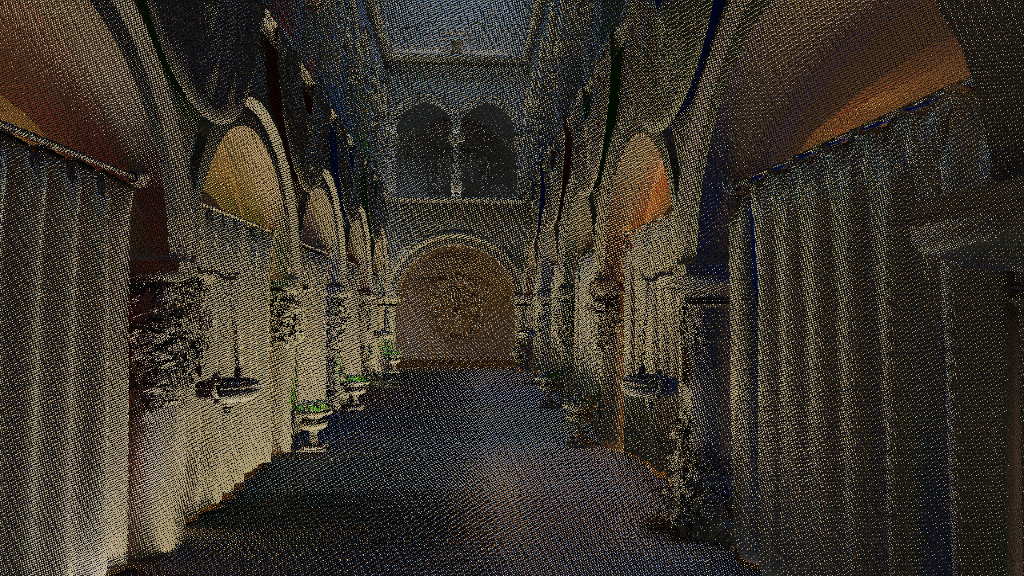
\includegraphics[width=\linewidth]{figures/gi_halfres.png}\\{\small polovi\v{c}na (0.5)}
\end{minipage}\hfill
\begin{minipage}{0.48\textwidth}\centering
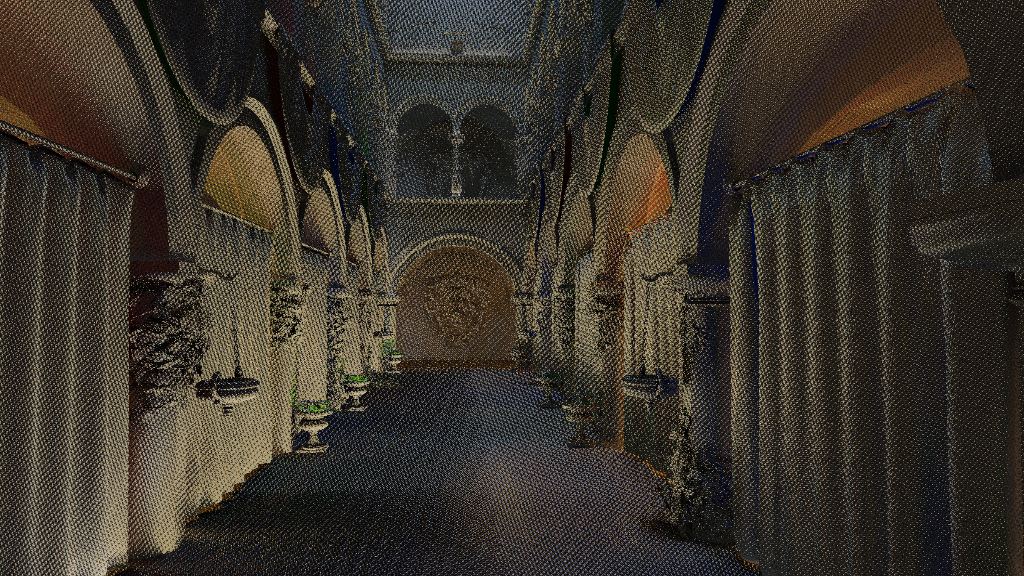
\includegraphics[width=\linewidth]{figures/gi_fullres.png}\\{\small puna (1.0)}
\end{minipage}
\caption[Sirov GI bafer: polovi\v{c}na naspram pune rezolucije]{Sirov GI bafer pre upsample-a i denoiser-a, pri \texttt{render.gi.scale} 0.5 i 1.0
(\texttt{render.debugview} 6). Puna rezolucija daje finiju zrnastost: 28.91 naspram 41.68 po meri
visokofrekventne energije. U finalnoj slici se ta razlika ne meri (Tabela~\ref{tab:halfres}).}
\label{fig:halfres-buffer}
\end{figure}

Two caveats bound that claim. The quality figures come from one viewpoint rather than the three-view
average used elsewhere, and the conclusion is specific to diffuse gather signals: as
Section~\ref{sec:rendergraph} argues, the same treatment applied to shadows or reflections would
destroy exactly the high-frequency detail those effects exist to produce, which is why neither is
traced at half resolution in the first place.

\section{Evaluacija denoiser-a (SVGF)}
\label{sec:denoise-eval}

The SVGF spatial denoiser's own contribution is isolated by holding temporal accumulation constant
(enabled in both states, settled over 90 frames) and scoring the noisy input against the denoised
result against the path-traced reference, at a fixed 2 rays per pixel, RX 9070 XT.

\begin{table}[htb]
\centering
\caption{Doprinos SVGF denoiser-a naspram path-traced reference (2 zraka/piksel, temporalni resolve
uklju\v{c}en u oba slu\v{c}aja).}
\label{tab:denoise-eval}
\begin{tabular}{@{}lrrr@{}}
\toprule
Denoiser & PSNR (dB) & SSIM & FLIP \\
\midrule
off & 24.67 & 0.7409 & 0.1446 \\
on & 24.65 & 0.7397 & 0.1449 \\
\bottomrule
\end{tabular}

\end{table}

With temporal accumulation already active, the spatial SVGF pass changes the static-frame metrics
(PSNR, SSIM, FLIP) by less than measurement noise: the temporal history is doing essentially all of
the visible convergence at this settled frame, and the filter's own contribution shows up in temporal
stability instead. A frame-to-frame RMS delta on the same static view (frame $N$ against $N{+}1$ at
steady state, a flicker proxy under a static camera, not motion) drops only from \flickerOff{} with
the denoiser off to \flickerOn{} with it on, a \flickerPct\% reduction. That figure is sensitive to
one protocol detail: unless temporal history is cleared before sampling, the unfiltered case is
credited with noise that accumulated while assets were still streaming, which inflates the apparent
reduction to near 40\%, so figures captured with and without that clear are not comparable. The
denoiser's GPU cost is read from its own timestamp scopes rather than from a whole-frame A/B: the
three \texttt{GIDenoise} à-trous iterations total \perfDenoiseAMD{} ms on the 9070 XT and
\perfDenoiseNV{} ms on the 5070 (Table~\ref{tab:pass-cost}), against a full-frame budget near nine
milliseconds, and they are cheap partly because they run at half resolution. Toggling the denoiser
and diffing whole-frame totals gives about 0.07 ms, which should not be quoted: it is smaller than
the run-to-run spread of the identical configuration, so it measures noise rather than the filter.

Debug views 6 and 7 isolate the filter from everything else in the image, showing the half-resolution
GI irradiance buffer as the trace leaves it and after temporal accumulation plus the à-trous, before
either is upsampled or composited (Figure~\ref{fig:gi-denoise-ab}). The high-frequency energy defined
in Section~\ref{sec:raycount} falls from \hfGiRaw{} to \hfGiDenoised{} between the two, some 96\% of
it, while the mean level rises because the filter fills in the pixels where every ray happened to
miss.

So the filter transforms the intermediate buffer almost completely, and yet the finished image is
unchanged to within measurement noise. The pipeline downstream absorbs the work: the buffer is
upsampled from half resolution, multiplied by surface albedo, added to direct lighting that dominates
it, then run through a temporal resolve that is itself a strong low-pass in time. At two rays per pixel with
temporal accumulation already active, the spatial à-trous is close to redundant for global
illumination and worse than redundant for reflections, which is why it is kept at three iterations
for the former and disabled for the latter rather than applied uniformly, and it argues for spending
a reconstruction budget on the temporal side before the spatial one.

\paragraph{Isti filtar na refleksijama je \v{s}tetan.} The same à-trous runs on the reflection signal
and there it measured net-negative, which is why it is now disabled by default: turning it off
improved every spatial metric at once, FLIP 0.1742 against 0.1746, PSNR 21.75 against 21.70, SSIM
0.6473 against 0.6419. That all three move the same way is what separates this from metric gaming,
since the signature of merely deleting blur is FLIP and PSNR improving while SSIM drops. The
structural reason is that the filter is guided by the receiving surface's normal and depth, correct
for a diffuse gather although wrong for reflections: reflected radiance is view-dependent, so on a
flat reflective surface those guides are constant and the kernel opens wide exactly where reflected
detail lives. The chain ran at full resolution with no upsample after it, so removing it is most of
the 1.1 ms by which reflections became cheaper in
Table~\ref{tab:cena}. A roughness-driven kernel remains the structurally right fix, although it now
has to beat filtering off rather than beat three iterations.

\paragraph{Cena filtra nije ista na oba proizvo\dj a\v{c}a.} Rolling the à-trous outer loop, done to
cut the shader's register pressure (Section~\ref{sec:occupancy}), paid asymmetrically: on the RTX
5070 every stride got faster, while on the RX 9070 XT it was close to a wash on the half-resolution
GI and AO chains (first iteration slower, last one faster) and paid only on the full-resolution ones.
The per-pass table shows the residue: the AMD denoise chain is front-loaded (\texttt{GIDenoise0}
0.133 ms falling to 0.089 ms at \texttt{GIDenoise2}) while the NVIDIA one inverts (0.094 ms rising to
0.127 ms). The stride-1 iteration is the one where adjacent taps are cache-friendly enough that
batching beats occupancy, and that tradeoff lands differently on the two memory hierarchies. A shader
optimisation justified by a register count is therefore not automatically a win, and has to be
measured per vendor like everything else in this chapter.

\begin{figure}[tbp]
\centering
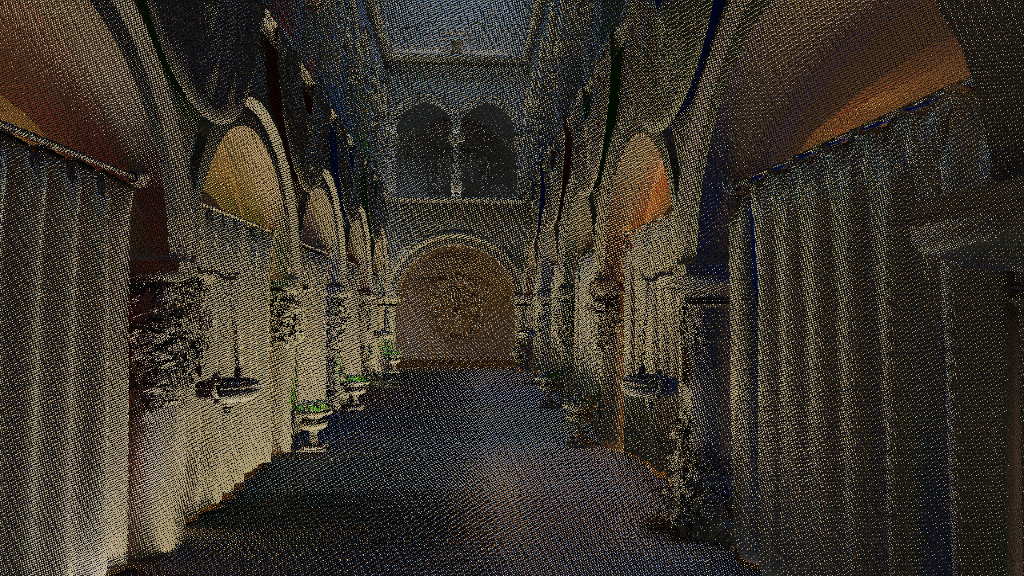
\includegraphics[width=0.48\textwidth]{figures/dbg_gi_raw.png}\hfill%
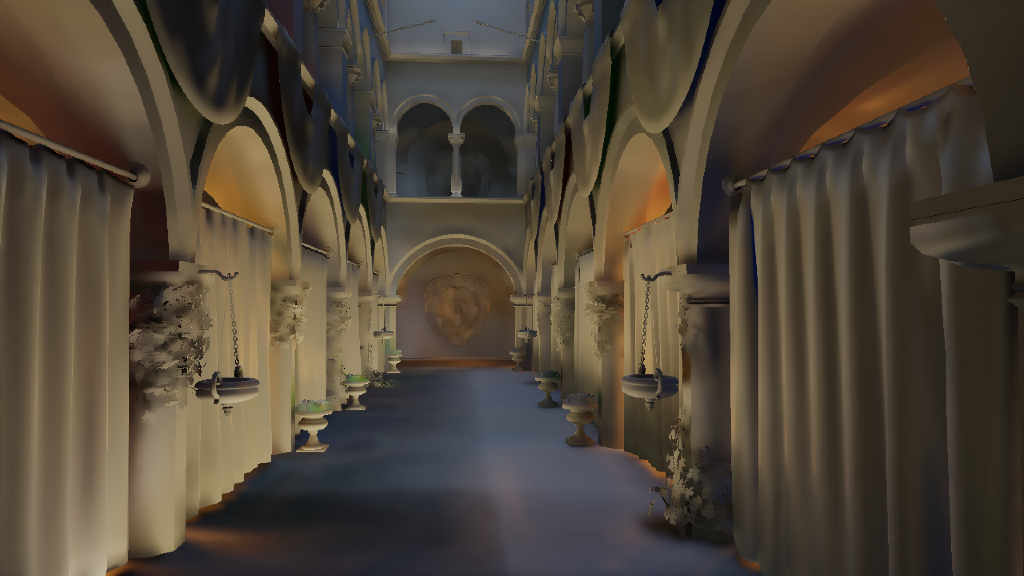
\includegraphics[width=0.48\textwidth]{figures/dbg_gi_denoised.png}
\caption{Polovi\v{c}na GI zra\v{c}nost pre (levo) i posle (desno) temporalne akumulacije i a-trous
filtra, pre upsample-a i kompozicije (\texttt{render.debugview} 6 i 7). Levo se vidi zrnasti
jednozra\v{c}ni signal, desno isti bafer nakon rekonstrukcije.}
\label{fig:gi-denoise-ab}
\end{figure}

\begin{figure}[tbp]
\centering
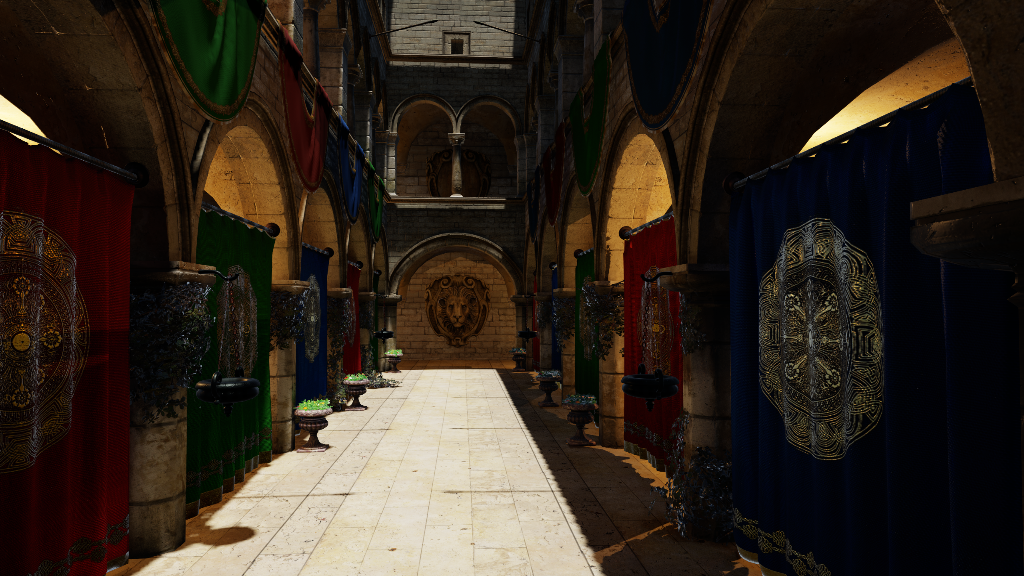
\includegraphics[width=0.62\textwidth]{figures/denoise_compare_noisy.png}

\vspace{5pt}

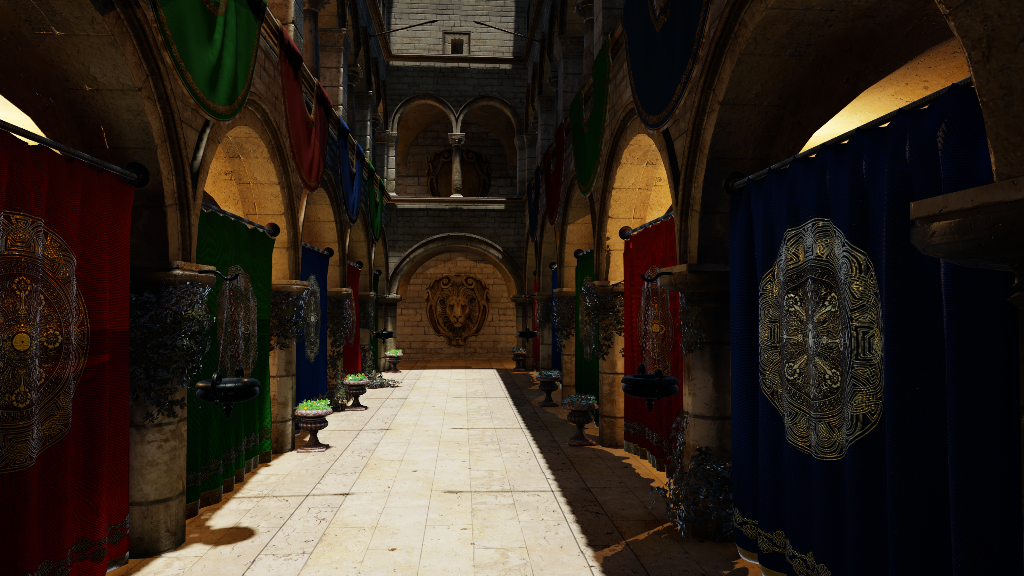
\includegraphics[width=0.62\textwidth]{figures/denoise_compare_denoised.png}

\vspace{5pt}

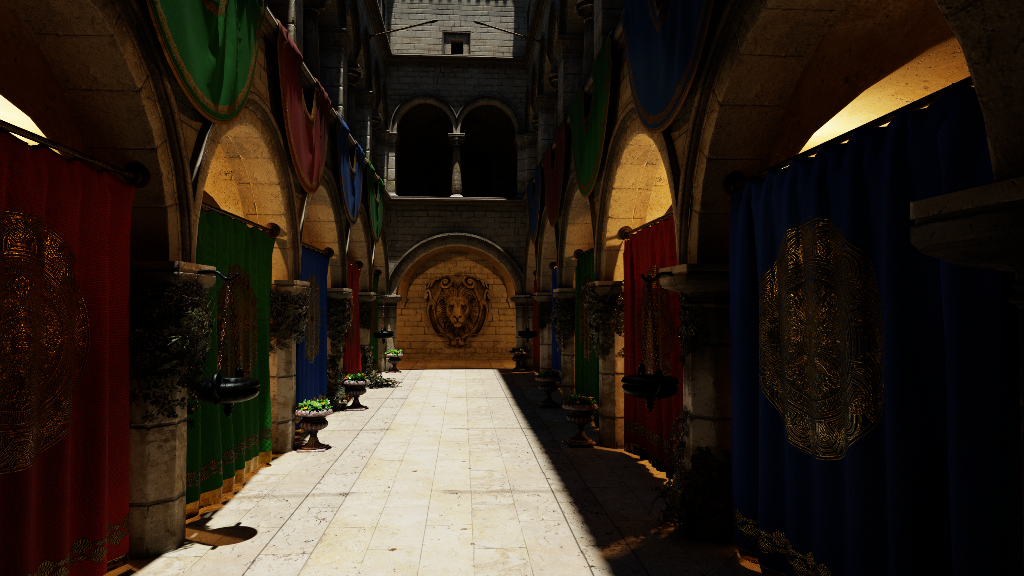
\includegraphics[width=0.62\textwidth]{figures/denoise_compare_reference.png}
\caption{Rekonstrukcija na 2 zraka po pikselu: sirov signal bez denoiser-a, temporalnog resolve-a i
TAA (gore), pun real-time rezultat sa sve tri komponente uklju\v{c}ene (sredina), i path-traced
referenca (dole). Razlika gore-sredina je doprinos cele rekonstrukcije; doprinos samog denoiser-a
izolovan je metrikama u tekstu, gde se vidi pre svega u temporalnoj stabilnosti.}
\label{fig:denoise-compare}
\end{figure}

\section{Pore\dj enje sa postoje\'cim re\v{s}enjima}
\label{sec:poredjenje}

The engine implements raster screen-space baselines for ambient occlusion and reflections (SSAO, SSR;
Section~\ref{sec:efekti}), so the comparison against the solutions surveyed in
Chapter~\ref{ch:pregled} is a same-scene, same-camera A/B, exposing the cases the screen-space method
structurally cannot handle: off-screen occluders and reflectors, and disocclusion
(Figure~\ref{fig:rt-vs-ss}). The positioning against production systems (Lumen, RTXGI, ReSTIR) is
qualitative: the contribution is an integrated, measured, openly licensed ray-query implementation,
not a system that beats a production global-illumination solution.

\begin{table}[tbp]
\caption{Kvalitet svake tehnike u odnosu na path-traced referencu (prosek preko tri pogleda: atrium,
floor, gallery; RX 9070 XT). Manji FLIP i ve\'ci PSNR/SSIM su bolji.}
\label{tab:quality}
\centering
\begin{tabular}{lrrr}
\toprule
Tehnika & FLIP $\downarrow$ & PSNR (dB) $\uparrow$ & SSIM $\uparrow$ \\
\midrule
raster (bez efekata) & 0.435 & 15.17 & 0.383 \\
SSAO                 & 0.418 & 15.61 & 0.398 \\
RT AO                & 0.414 & 15.71 & 0.400 \\
SSR                  & 0.429 & 15.31 & 0.395 \\
RT refleksije        & 0.422 & 15.44 & 0.404 \\
SSGI                 & 0.341 & 17.56 & 0.457 \\
RT GI                & 0.141 & 25.21 & 0.720 \\
sve RT (all-RT)      & \textbf{0.086} & \textbf{30.85} & \textbf{0.872} \\
\bottomrule
\end{tabular}

\end{table}

\begin{figure}[tbp]
\centering
\begin{tikzpicture}
\begin{axis}[width=0.88\textwidth, height=6.2cm,
  ylabel={FLIP $\downarrow$}, ymin=0, ymax=0.58,
  xtick={0,...,7},
  xticklabels={raster,SSAO,RT AO,SSR,RT refl.,SSGI,RT GI,sve RT},
  xticklabel style={font=\small, rotate=25, anchor=north east},
  tick label style={font=\small}, label style={font=\small},
  grid=major, grid style={black!12}, enlarge x limits=0.08]
\addplot[only marks, mark=*, mark size=2pt, black,
  error bars/.cd, y dir=both, y explicit]
  table[col sep=tab, x=i, y=flip, y error plus expr=\thisrow{hi}-\thisrow{flip},
        y error minus expr=\thisrow{flip}-\thisrow{lo}] {data/quality-spread.dat};
\end{axis}
\end{tikzpicture}
\caption[FLIP po tehnici sa rasipanjem po pogledima]{Isti podaci kao
Tabela~\ref{tab:quality}, ali sa rasponom preko tri pogleda umesto samo proseka. Rasipanje je deo
rezultata: raster se kre\'ce od 0.363 do 0.534 zavisno od kadra, dok se RT GI dr\v{z}i u 0.129--0.149.
Tehnike koje re\v{s}avaju indirektno osvetljenje nisu samo ta\v{c}nije u proseku, nego i ujedna\v{c}enije
po sceni, \v{s}to prosek sam ne pokazuje.}
\label{fig:quality-spread}
\end{figure}

Against the path-traced reference (Table~\ref{tab:quality}) global illumination is the dominant
quality lever: RT GI alone lifts
PSNR from \qRasterPsnr{} (raster) to \qRtGiPsnr{} and cuts FLIP by more than two thirds, and enabling
all effects reaches FLIP \qAllRtFlip{}, PSNR \qAllRtPsnr{}, SSIM \qAllRtSsim{}, by far the closest to
the reference. At these
whole-frame metrics screen-space and ray-traced AO and reflections are near-parity (SSAO versus RT AO,
and SSR versus RT reflections, differ by under 0.01 in FLIP), because the occlusion and reflection
contributions are small at the whole-frame level. Captured through the debug view that isolates the
AO term alone, the atrium viewpoint has a median AO
of 255 of 255, that is no occlusion at all, and only 14.1\% (SSAO) and 17.6\% (RT AO) of pixels fall
below 240. An effect that leaves five sixths of the frame untouched cannot move a whole-frame average
much, whichever way it is computed. The ray-traced advantage is off-screen correctness, which a
whole-frame average does not isolate; Figure~\ref{fig:ssvsrt-refl} isolates it for reflections by
showing the reflection buffer itself instead of the composited frame. Screen-space GI sits between those two tiers: its FLIP (0.341) is markedly better than
the AO/reflection pairs but well short of RT GI (0.141), consistent with SSGI only gathering bounce
light from on-screen geometry, where RT GI also reaches off-screen and behind-camera surfaces.

\begin{figure}[tbp]
\centering
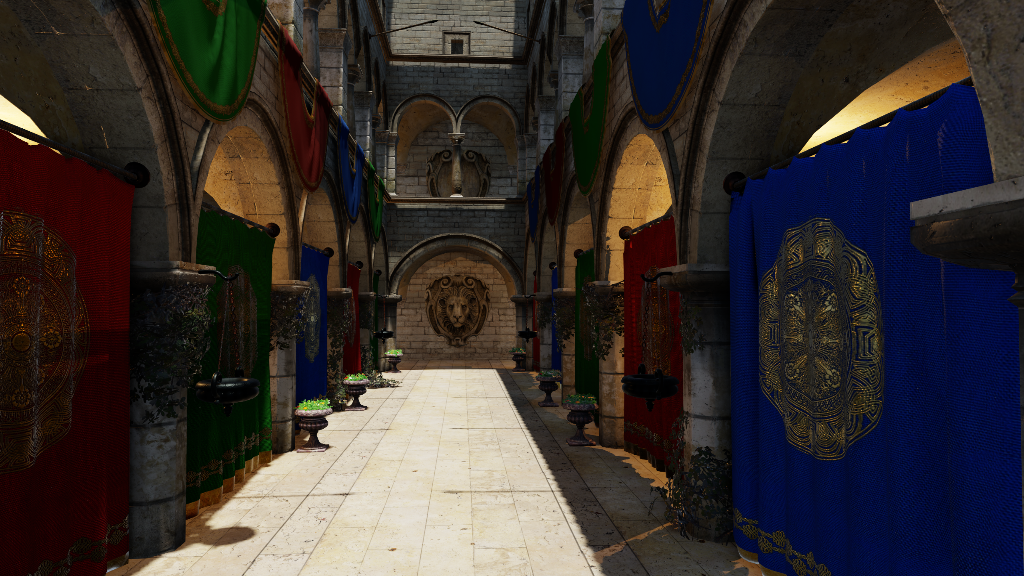
\includegraphics[width=0.48\textwidth]{figures/ss_all.png}\hfill%
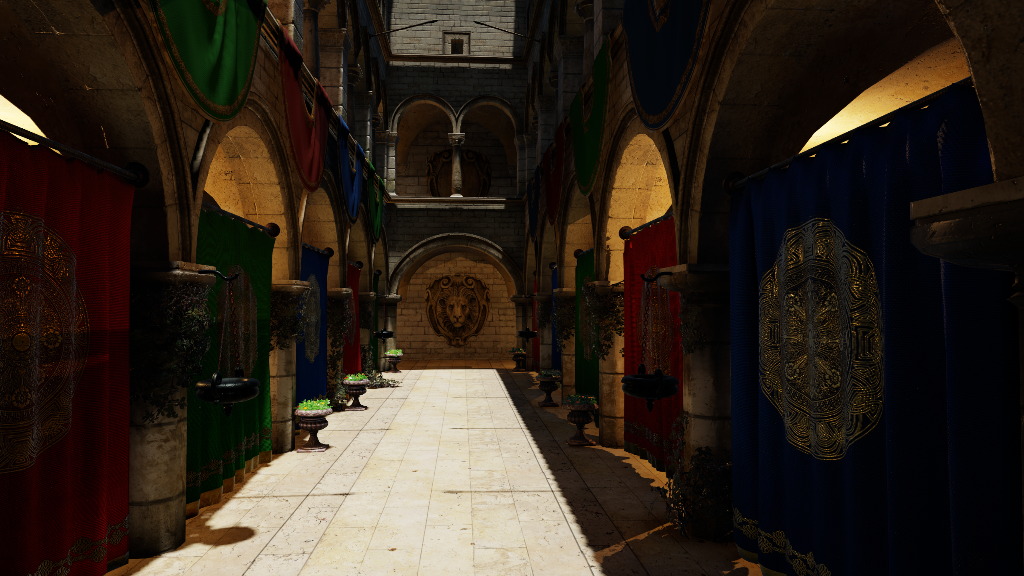
\includegraphics[width=0.48\textwidth]{figures/rt_all.png}
\caption[Screen-space naspram ray-traced konfiguracije]{Ista scena i kamera, dve celovite
konfiguracije: screen-space (levo: mapa senki, SSAO, SSR, SSGI) naspram ray-traced (desno: trasirane
senke, RTAO, RT refleksije, RT GI). Senke prate ostatak jer screen-space nema svoj pandan trasiranoj
senci, pa je mapa ono \v{s}to ta familija zaista koristi; to je ista podela koju koristi i red
\rqt{sve RT} u Tabeli~\ref{tab:quality}. Screen-space varijanta je svetlija jer ne mo\v{z}e da oduzme
svetlo koje dolazi od geometrije van ekrana.}
\label{fig:rt-vs-ss}
\end{figure}

\begin{figure}[tbp]
\centering
\begin{minipage}{0.48\textwidth}\centering
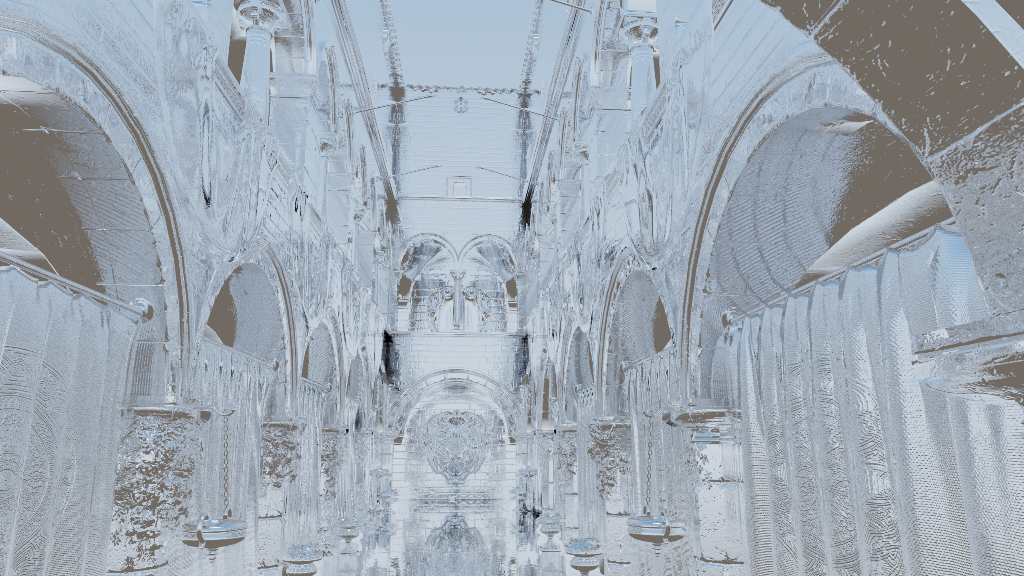
\includegraphics[width=\linewidth]{figures/ssvsrt_ssr.png}\\{\small SSR}
\end{minipage}\hfill
\begin{minipage}{0.48\textwidth}\centering
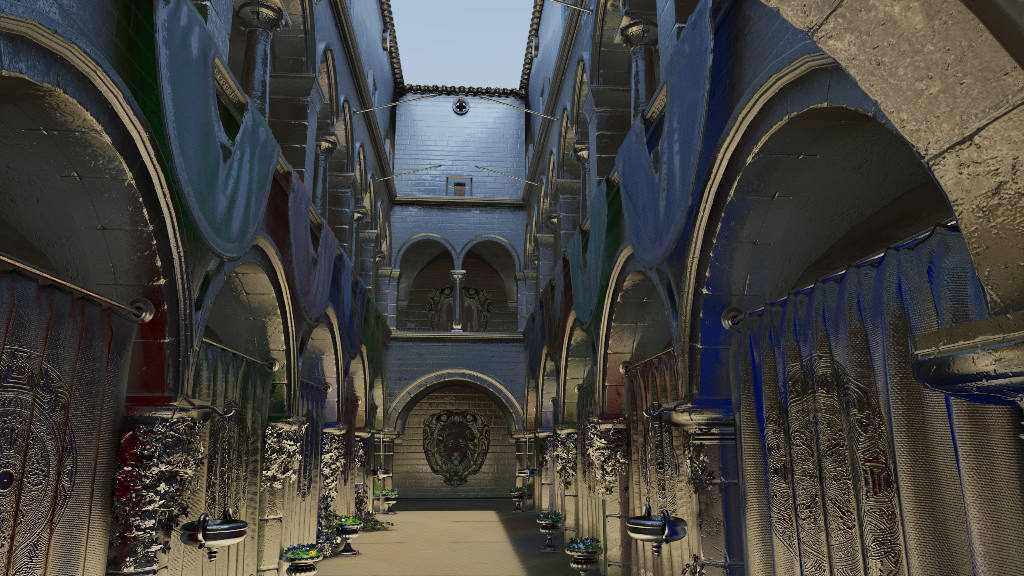
\includegraphics[width=\linewidth]{figures/ssvsrt_rtrefl.png}\\{\small RT refleksije}
\end{minipage}
\caption[Sirov bafer refleksije: SSR naspram RT]{Sirov bafer refleksije (\texttt{render.debugview} 3),
isti pogled i iste podrazumevane vrednosti; SSR i RT pi\v{s}u u isti bafer, pa je jedina promenljiva
izvor refleksije. Kada mar\v{s} kroz dubinski bafer ne na\dj e ni\v{s}ta, SSR vra\'ca prefiltriranu
mapu okru\v{z}enja: 9.0\% piksela je zbog toga skoro belo, naspram 0.0\% na desnoj strani, a srednja
vrednost bafera je 169.4 naspram 65.99. U slo\v{z}enom kadru se ta razlika gubi ispod direktnog
osvetljenja, zbog \v{c}ega je FLIP dve tehnike gotovo isti.}
\label{fig:ssvsrt-refl}
\end{figure}

\section{Stabilnost pod kretanjem}
\label{sec:motion}

Every quality figure so far comes from a static camera, which Section~\ref{sec:denoise-eval} found
hides most of what the spatial denoiser does: it cuts frame-to-frame flicker by \flickerPct\% while
moving the static metrics by less than measurement noise, an argument made there only by proxy. This
section moves the camera.

Flying a fixed route, capturing frames along it and scoring each against a converged path trace of
the same instant produces a caution about the method before any fact about the renderer: across the
eleven techniques, the per-frame FLIP measured this way correlates with the static FLIP of
Section~\ref{sec:poredjenje} at $r = +0.99$, very nearly the same measurement taken twice. A
converged per-frame path trace is a sequence of independent still images with no temporal structure,
since nothing in its construction relates one frame to the next, so error measured against it has no
temporal component to carry however much the camera moves. The defect is in that experimental design
rather than in the implementation, and it is a known conflation: k-DOP Clipping
\cite{ikkala2024kdop} states outright that a supersampled reference introduces a constant error by
also comparing general temporal-antialiasing quality against supersampling. The canonical denoiser
papers avoid it by reporting accuracy against a reference and temporal behaviour separately, the
latter with a reference-free measure.

Two quantities in the moving capture do carry information the static gate cannot. The first compares
how much the technique changes between consecutive frames against how much the \emph{reference}
changes over the same interval, so that motion inherent to the scene is subtracted and only excess
instability remains. Subtracting matters: on this route the reference itself moves by a FLIP of about
0.09 between adjacent frames, which a naive frame difference would report as instability. Ranked by
it (Table~\ref{tab:motion}), the techniques order exactly as the flicker proxy predicted, the fully
reconstructed configurations most stable and plain rasterization least, which is
Section~\ref{sec:denoise-eval}'s conclusion reached under motion instead of by proxy: the spatial
filter buys stability rather than static fidelity. The two temporal metrics disagree usefully:
\texttt{rtgi} has the best tFLIP while \texttt{all-rt} has the best JOD, because tFLIP isolates
temporal excess alone where ColorVideoVDP is spatio-temporal and \texttt{all-rt} is far more accurate
spatially.

\begin{table}[tbp]
\caption[Stabilnost pod kretanjem po tehnici]{Stabilnost pod kretanjem, prosek preko \v{c}etiri probne
ta\v{c}ke rute (RX 9070 XT), pore\dj ano po FLIP-u. tFLIP meri koliko se tehnika menja izme\dj u
susednih kadrova preko onoga koliko se menja sama referenca; ka\v{s}njenje je pokretni kadar naspram
sopstvenog konvergiranog mirnog kadra u istoj pozi. JOD je ColorVideoVDP, jedina mera ovde koja
direktno modeluje vremensku osetljivost.}
\label{tab:motion}
\centering
\begin{tabular}{lrrrr}
\toprule
Tehnika & FLIP $\downarrow$ & tFLIP $\downarrow$ & ka\v{s}njenje $\downarrow$ & JOD $\uparrow$ \\
\midrule
sve RT (all-RT)                  & 0.173 & 0.0082 & 0.104 & 4.81 \\
RT GI                            & 0.208 & 0.0081 & 0.119 & 3.89 \\
SSGI                             & 0.293 & 0.0161 & 0.129 & 3.28 \\
stohasti\v{c}ke senke (bez spec.) & 0.328 & 0.0120 & 0.126 & 3.18 \\
RT senke                         & 0.329 & 0.0154 & 0.120 & 3.22 \\
stohasti\v{c}ke senke            & 0.330 & 0.0127 & 0.127 & 3.16 \\
RT AO                            & 0.343 & 0.0198 & 0.124 & 3.25 \\
SSAO                             & 0.346 & 0.0198 & 0.123 & 3.16 \\
RT refleksije                    & 0.347 & 0.0162 & 0.120 & 3.17 \\
SSR                              & 0.362 & 0.0203 & 0.125 & 3.09 \\
raster                           & 0.362 & 0.0205 & 0.124 & 3.05 \\
\bottomrule
\end{tabular}

\end{table}

The second is lag: the moving frame scored against this renderer's own converged still at the same
pose, which measures how far reconstruction trails the camera, read across the route in
Table~\ref{tab:motion-probes} for the two ends of the ranking. Velocity reversal is the costliest
motion, and not because of speed, since the route holds translation essentially constant: what is
special about a reversal is that the velocity vector changes sign, the documented pathological case
for history rejection. The parked probe is an order of magnitude below the moving ones and acts as
the control that makes them readable.

\begin{table}[tbp]
\caption[Stabilnost i ka\v{s}njenje po ta\v{c}ki rute]{Iste dve vremenske mere razlo\v{z}ene po
probnim ta\v{c}kama, za krajeve rangiranja. Vrednosti se ne porede izme\dj u kolona: svaka ta\v{c}ka
gleda drugi sadr\v{z}aj, pa je razlika me\dj u njima uglavnom razlika u onome \v{s}to je na ekranu.}
\label{tab:motion-probes}
\centering
\begin{tabular}{llrrrr}
\toprule
Technique & metric & dolly & strafe & reversal & parked \\
\midrule
raster & tFLIP & 0.0193 & 0.0319 & 0.0270 & 0.0036 \\
raster & lag & 0.120 & 0.175 & 0.185 & 0.016 \\
all RT (all-RT) & tFLIP & 0.0137 & 0.0161 & 0.0010 & 0.0019 \\
all RT (all-RT) & lag & 0.089 & 0.138 & 0.166 & 0.024 \\
\bottomrule
\end{tabular}

\end{table}

Three cautions belong with these numbers. They must not be compared across probes as if the probes
were equally hard, because each looks at different scene content: plain rasterization scores its
\emph{best} per-frame FLIP on the reversal probe while showing its worst lag there. The lag measure is
this renderer against its own still, so it can be driven to zero by degrading the still and must never
be used as an optimisation target. And its absolute scale depends on the capture protocol, which was
corrected during this work, so only figures from the current baselines may be quoted and never mixed
with earlier ones.

\section{Kvalitet izme\dj u proizvo\dj a\v{c}a}
\label{sec:cross-vendor-quality}

The cross-vendor argument rests on the two adapters running identical code, which elsewhere justifies
comparing \emph{time}. If the reconstructed images did not also agree, a timing difference could
always be dismissed as the two cards having done different amounts of work.

The whole quality matrix was captured a second time on the RTX 5070, giving 33 viewpoint and technique
pairs. Across all 33 the largest absolute difference in FLIP between the adapters is \textbf{0.0037},
the median is \textbf{0.0007}, and 24 of the 33 fall below 0.001. The secondary metrics agree to the
same degree: PSNR never differs by more than 0.10 dB and SSIM never by more than 0.0045. For scale,
the difference this chapter is actually interested in, between raster and all effects enabled, is a
FLIP of \qRasterFlip{} against \qAllRtFlip{}, two orders of magnitude larger than the vendor
disagreement.

Technique quality is therefore effectively vendor-independent here, so the entire
cross-vendor story of this thesis is cost rather than image quality:
the per-effect timings in Section~\ref{sec:cena} and the shadow-strategy inversion in
Section~\ref{sec:analiza-shadow-strategy} can be read as pure performance differences, with no
accompanying quality caveat.

Both adapters are scored against the \emph{same} path-traced reference, and the obvious alternative
would have destroyed the result. The
reference cache is keyed on the scene, the camera pose, the frame count and the content of the
path-tracing shaders, and deliberately not on the device, so the second adapter reuses the reference
the first produced rather than tracing its own. Had each been scored against a reference it produced
itself, every comparison would have carried the difference between two independently converged path
traces, and there is no reason to assume that difference is small next to the technique difference
being measured. Sharing the reference makes the reference error common to both sides, where it
cancels.

Two limits bound the claim. The residual disagreement is not zero, and the largest of it sits on the
ambient-occlusion and shadow rows, which are also the effects whose rays interact with the cutout
geometry where the two drivers genuinely differ (Section~\ref{sec:metodologija}). That is consistent
with the opacity-micromap disparity being the mechanism, although this experiment does not isolate it.
And the reference is shared here because both adapters were measured on one machine with a warm cache;
on two machines each would trace its own, and the comparison would require transferring the reference
rather than recomputing it.

\section{Zauzetost i cena \v{s}ejdera}
\label{sec:occupancy}

Static shader occupancy, how many registers each ray-tracing and denoising shader needs and how many
waves the hardware can therefore keep in flight, is the one place where the two vendors compare on
something other than time, and it explains part of the cost difference the rest of the chapter
measures.

Two artifacts feed it, with deliberately different authority. For AMD the offline analyser compiles
every shader and permutation, so its coverage is complete and deterministic, and it is what the
project gates on. For NVIDIA no offline analyser exists, since register allocation happens inside the
driver's just-in-time compiler, so those figures are read back from the driver through
\texttt{VK\_KHR\_pipeline\_executable\_properties} after the pipelines are built. The two agree on
every AMD register count they share, which is what licenses carrying the offline permutation labels
over to the runtime numbers: the runtime capture reports both \texttt{DefaultLit} variants under one
pipeline name and cannot tell them apart on its own.

\begin{table}[tbp]
\caption{Registri i teorijska zauzetost klju\v{c}nih \v{s}ejdera na oba GPU-a. Za AMD: broj VGPR-a i
najve\'ci mogu\'ci broj wave32 talasa po SIMD-u (1536 VGPR-a, granularnost 24, najvi\v{s}e 16). Za
NVIDIA: broj registara po niti i najve\'ci broj warp-ova po SM-u (65536 registara, najvi\v{s}e 48).
Obe vrednosti su teorijske i izvedene iz broja registara, ne izmerene profajlerom. Generi\v{s}e se iz
committovanih baseline-a skriptom \texttt{tools/gen\_shader\_tables.py}.}
\label{tab:occupancy}
\centering
\begin{tabular}{lrrrr}
\toprule
& \multicolumn{2}{c}{RX 9070 XT (RDNA4)} & \multicolumn{2}{c}{RTX 5070 (Blackwell)} \\
\cmidrule(lr){2-3}\cmidrule(lr){4-5}
\v{S}ejder & VGPR & talasa/SIMD & registara & warp-ova/SM \\
\midrule
\texttt{DefaultLit.frag} (inline senke) & 127 & 10/16 & 80 & 25/48 \\
\texttt{DefaultLit.frag} (bez inline senki) & 87 & 16/16 & 64 & 32/48 \\
\texttt{GI.comp} & 83 & 16/16 & 64 & 32/48 \\
\texttt{Reflection.comp} & 81 & 16/16 & 64 & 32/48 \\
\texttt{AO.comp} & 60 & 16/16 & 48 & 42/48 \\
\texttt{GIDenoise.comp} (GI) & 59 & 16/16 & 48 & 42/48 \\
\bottomrule
\end{tabular}

\end{table}

Only one shader on the render path is occupancy-limited on either card, and it is the same one:
\texttt{DefaultLit.frag} in its inline-shadow permutation, at 127 VGPRs and 10 of 16 waves on the
9070 XT. Compiled without the inline shadow query it drops to 87 VGPRs and full occupancy, which
locates the cost precisely: tracing shadow rays inside the forward shader is what pushes it over a
wave boundary, the same effect Section~\ref{sec:cena} sees as a Forward pass that grows by 3.482 ms.
Nothing in the table spills registers, and across all 47 cooked shaders exactly one uses scratch
memory at all (\texttt{NeuralConv.comp}, 272 bytes), off the render path.

Figure~\ref{fig:occupancy-cliff} plots why the two permutations land so far apart for a difference of
40 registers. Occupancy is a step function of register use, since registers are allocated in fixed
blocks of 24 on this architecture and the wave count is the register file divided by that rounded-up
allocation. Between 24 and 96 VGPRs every shader gets all 16 waves, so the five shaders in the flat
region differ in register use by a factor of 1.5 (59 to 87) at no cost in parallelism. Past 96 the
count falls in steps: the inline-shadow permutation at 127 VGPRs allocates 144 and gets 10 waves; had
it stayed at or below 96, as its non-tracing sibling does at 87, it would have cost nothing. Hence gating
on occupancy rather than on the register count directly, and acting on a register increase only when
it crosses a step.

\begin{figure}[tbp]
\centering
\begin{tikzpicture}
\begin{axis}[width=0.86\textwidth, height=6.2cm,
  xlabel={VGPR-a po niti}, ylabel={talasa po SIMD-u (wave32)},
  xmin=24, xmax=192, ymin=0, ymax=17.5,
  ytick={0,4,8,12,16}, xtick={24,48,72,96,120,144,168,192},
  grid=major, grid style={black!12}, tick label style={font=\small},
  label style={font=\small}]
  \addplot[const plot, thick, black] table[col sep=tab, x=vgpr, y=waves] {data/occupancy-curve.dat};
  \addplot[only marks, mark=*, mark size=1.9pt, black]
    table[col sep=tab, x=vgpr, y=waves] {data/occupancy-marks.dat};
  \node[font=\footnotesize, anchor=west] at (axis cs:130,10.9) {\texttt{DefaultLit} (inline senke)};
  \node[font=\footnotesize, anchor=east] (nobez) at (axis cs:80,13.6) {\texttt{DefaultLit} (bez)};
  \draw[black!55, thin] (nobez.east) -- (axis cs:87,15.6);
\end{axis}
\end{tikzpicture}
\caption[Zauzetost kao stepenasta funkcija broja VGPR-a]{Teorijska zauzetost kao stepenasta funkcija broja VGPR-a na RDNA4 (1536 VGPR-a,
granularnost 24, najvi\v{s}e 16 talasa). Ta\v{c}ke su \v{s}ejderi iz Tabele~\ref{tab:occupancy}. Do 96
VGPR-a razlika u broju registara ne ko\v{s}ta ni\v{s}ta; \texttt{DefaultLit} sa inline senkama pada
preko granice na 127.}
\label{fig:occupancy-cliff}
\end{figure}

The cross-vendor comparison inverts the naive reading. NVIDIA uses markedly fewer registers for the
same shader, 80 against 127 for the inline-shadow variant, yet its relative occupancy is \emph{lower},
25 of 48 warps against 10 of 16 waves (52\% against 62\%), because of the ratio each architecture
provides: a Blackwell SM has 65536 registers for up to 48 warps of 32 threads, about 42 registers per
thread at full occupancy, so pressure begins to bite earlier there than the raw counts suggest. Fewer
registers used does not mean more parallelism available.

Three limits belong with these numbers. The occupancy is theoretical and register-derived, so it is an
upper bound on both vendors and says nothing about what is achieved once memory stalls and other
limits are included; that needs a runtime profiler. The RDNA4 register allocation granularity is taken
from documentation and has not been confirmed against a per-compile report the way the RDNA3 figure
was, so a wave count sitting near a boundary is model-dependent: at a granularity of 8 rather than 24
the inline-shadow permutation would read 12 of 16 rather than 10. And the NVIDIA figure is explicitly
an upper bound, since the allocation granularity for that compute capability is not published and
rounding up can only lower the warp count.

Register spilling on NVIDIA is deliberately not reported: the driver returns a \texttt{Local Memory
Size} whose upper 32 bits are a constant, so the values differ only in their low half, and while that
low half is very likely the real figure, masking it would be inference presented as measurement.
